\documentclass{article}

\usepackage[francais]{babel}
\usepackage[T1]{fontenc}
\usepackage[latin1]{inputenc}
\usepackage[left=1cm, right=1cm, top=6mm, bottom=6mm]{geometry}
\usepackage{float}
\usepackage{graphicx}
\usepackage{array}
\usepackage{multirow}
\usepackage{amsmath, amssymb, mathrsfs}

\begin{document}

\begin{flushleft}
NOM PRENOM: \ldots \ldots \ldots \ldots \ldots \ldots \ldots \ldots \ldots

\bigskip
\end{flushleft}
\begin{center}
{\fbox{$2^{de}5$ \qquad \qquad \textbf{\Large{Contr�le de cours 5 (sujet 1)}}
\qquad \qquad 03/04/2009}}
\end{center}


\bigskip

\textbf{Exercice 1:} Pour chacune des droites suivantes, d�terminer son
�quation (vous laisserez apparent vos calculs et/ou traits de constructions).

\medskip

\begin{tabular}{cc}
\begin{minipage}{10cm}
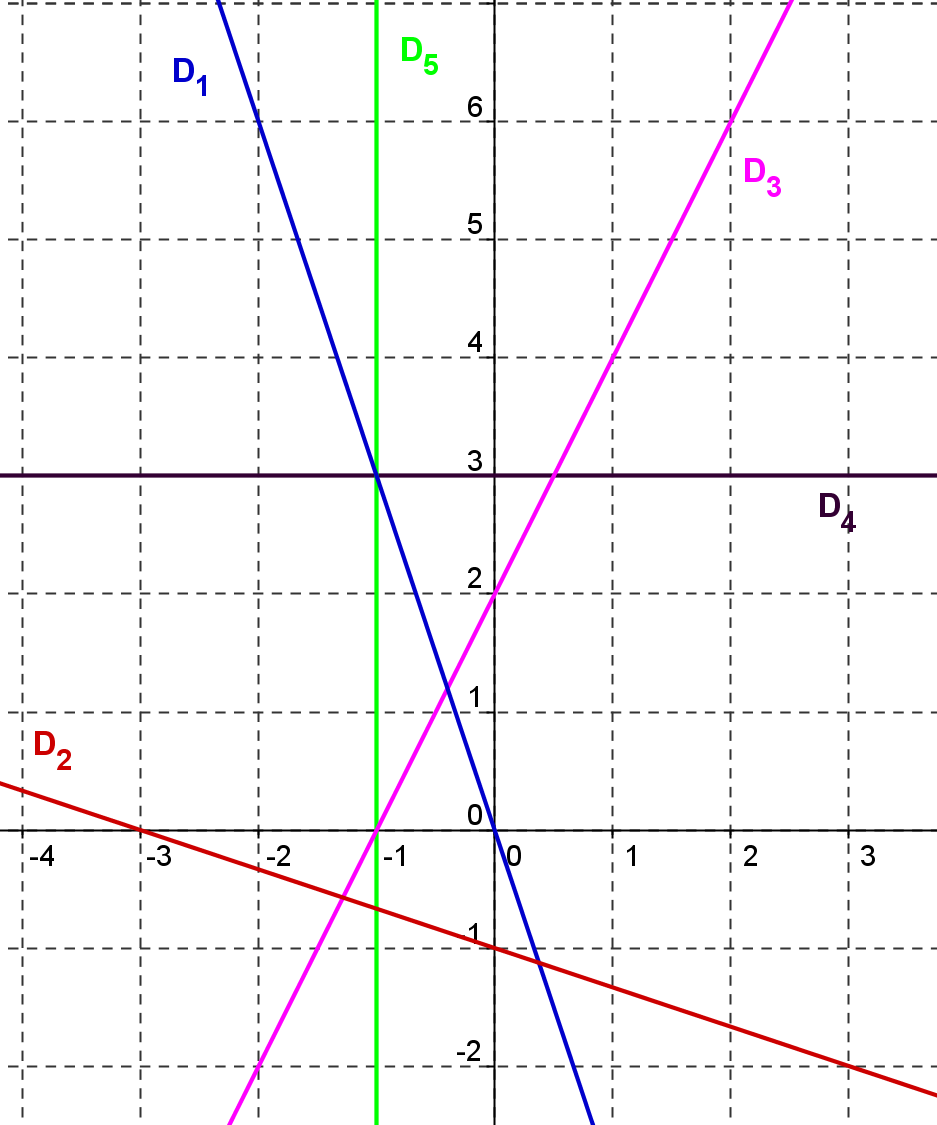
\includegraphics[width=7cm]{images/ex11.png}

\end{minipage}
&
\begin{minipage}{8cm}

\begin{tabular}{|c|c|}
\hline
 \qquad & \quad \\
\textbf{Droites} & \textbf{Equations} \\
\quad & \quad \\
\hline

\qquad & \quad \\
$D_1$ &    \qquad \qquad \qquad \qquad  \qquad \qquad \qquad         \\
\qquad & \quad \\
\hline
\qquad & \quad \\
$D_2$ &                \\
\qquad & \quad \\
\hline
\qquad & \quad \\
$D_3$ &                 \\
\qquad & \quad \\
\hline
\qquad & \quad \\
$D_4$ &                 \\
\qquad & \quad \\
\hline
\qquad & \quad \\
$D_5$ &                   \\
\qquad & \quad \\
\hline 
\end{tabular}



\end{minipage}
\end{tabular}


\bigskip

\textbf{Exercice 2} 


\begin{enumerate}
  \item Tracer en rouge la repr�sentation graphique de la fonction
  $f(x)=\dfrac{-2}{5}x+3$.
  \item Tracer en bleu la repr�sentation graphique de la fonction affine $g$ tel
  que:
  
  
 $\bullet$ le point $A(-1;2)$ appartient � la courbe repr�sentative de $g$
  
  
  $\bullet$ le coefficient directeur est 3.
  
  
(vous laisserez apparent vos calculs et/ou traits de constructions)
\end{enumerate}

\medskip

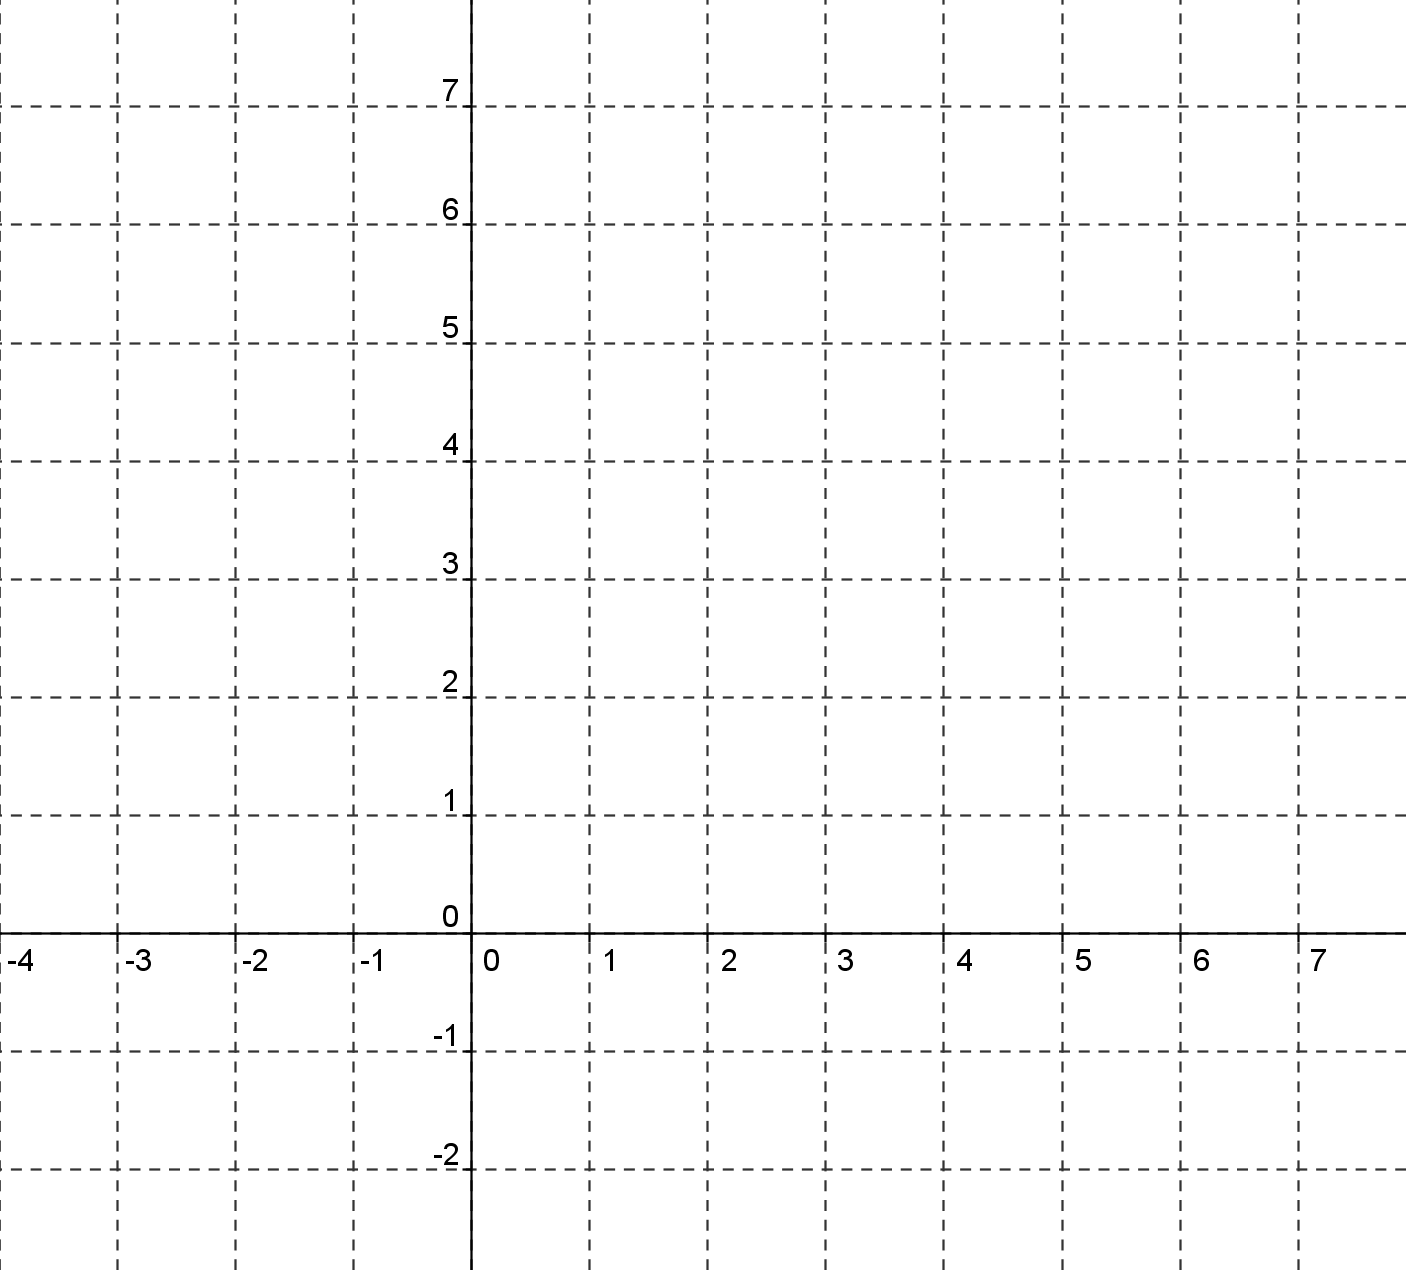
\includegraphics[width=12cm]{images/ex2.png}   

\pagebreak

\begin{flushleft}
NOM PRENOM: \ldots \ldots \ldots \ldots \ldots \ldots \ldots \ldots \ldots

\bigskip
\end{flushleft}
\begin{center}
{\fbox{$2^{de}5$ \qquad \qquad \textbf{\Large{Contr�le de cours 5 (sujet 2)}}
\qquad \qquad 03/04/2009}}
\end{center}


\bigskip

\textbf{Exercice 1:} Pour chacune des droites suivantes, d�terminer son
�quation (vous laisserez apparent vos calculs et/ou traits de constructions).

\medskip

\begin{tabular}{cc}
\begin{minipage}{10cm}
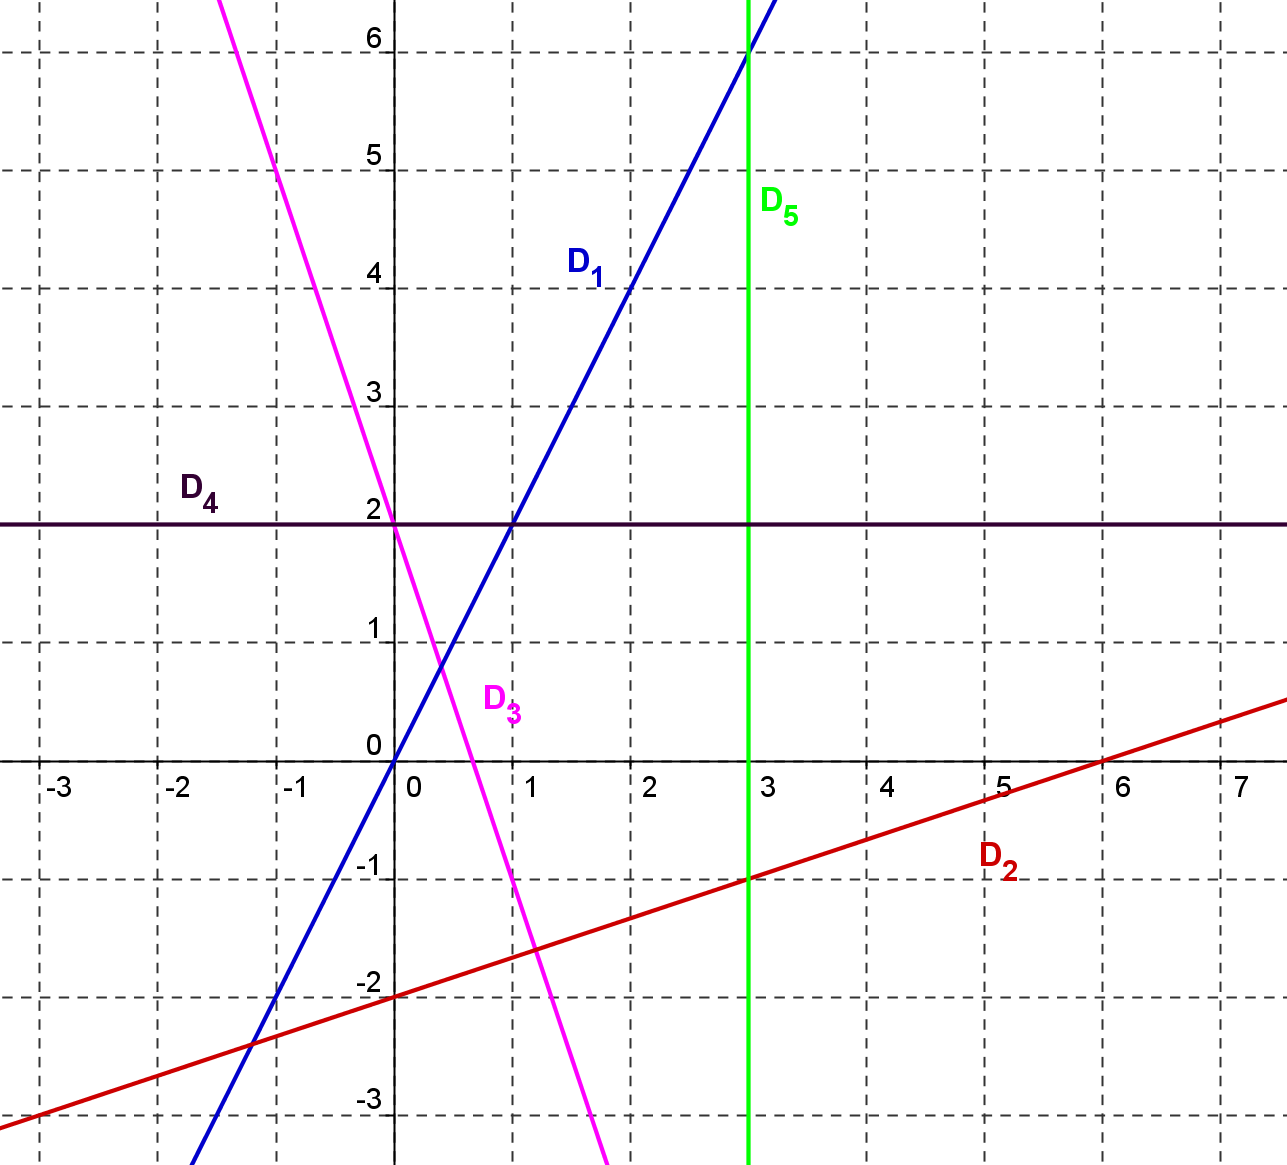
\includegraphics[width=9cm]{images/ex12.png}

\end{minipage}
&
\begin{minipage}{8cm}
 
\begin{tabular}{|c|c|}
\hline
 \qquad & \quad \\
\textbf{Droites} & \textbf{Equations} \\
\quad & \quad \\
\hline

\qquad & \quad \\
$D_1$ &    \qquad \qquad \qquad \qquad  \qquad \qquad \qquad         \\
\qquad & \quad \\
\hline
\qquad & \quad \\
$D_2$ &                \\
\qquad & \quad \\
\hline
\qquad & \quad \\
$D_3$ &                 \\
\qquad & \quad \\
\hline
\qquad & \quad \\
$D_4$ &                 \\
\qquad & \quad \\
\hline
\qquad & \quad \\
$D_5$ &                   \\
\qquad & \quad \\
\hline 
\end{tabular}



\end{minipage}
\end{tabular}


\bigskip

\textbf{Exercice 2} 


\begin{enumerate}
  \item Tracer en rouge la repr�sentation graphique de la fonction
  $f(x)=\dfrac{4}{3}x+1$.
  \item Tracer en bleu la repr�sentation graphique de la fonction affine $g$ tel
  que:
  
  
 $\bullet$ le point $A(1;2)$ appartient � la courbe repr�sentative de $g$
  
  
  $\bullet$ le coefficient directeur est -2.
  
(vous laisserez apparent vos calculs et/ou traits de constructions)
\end{enumerate}

\medskip

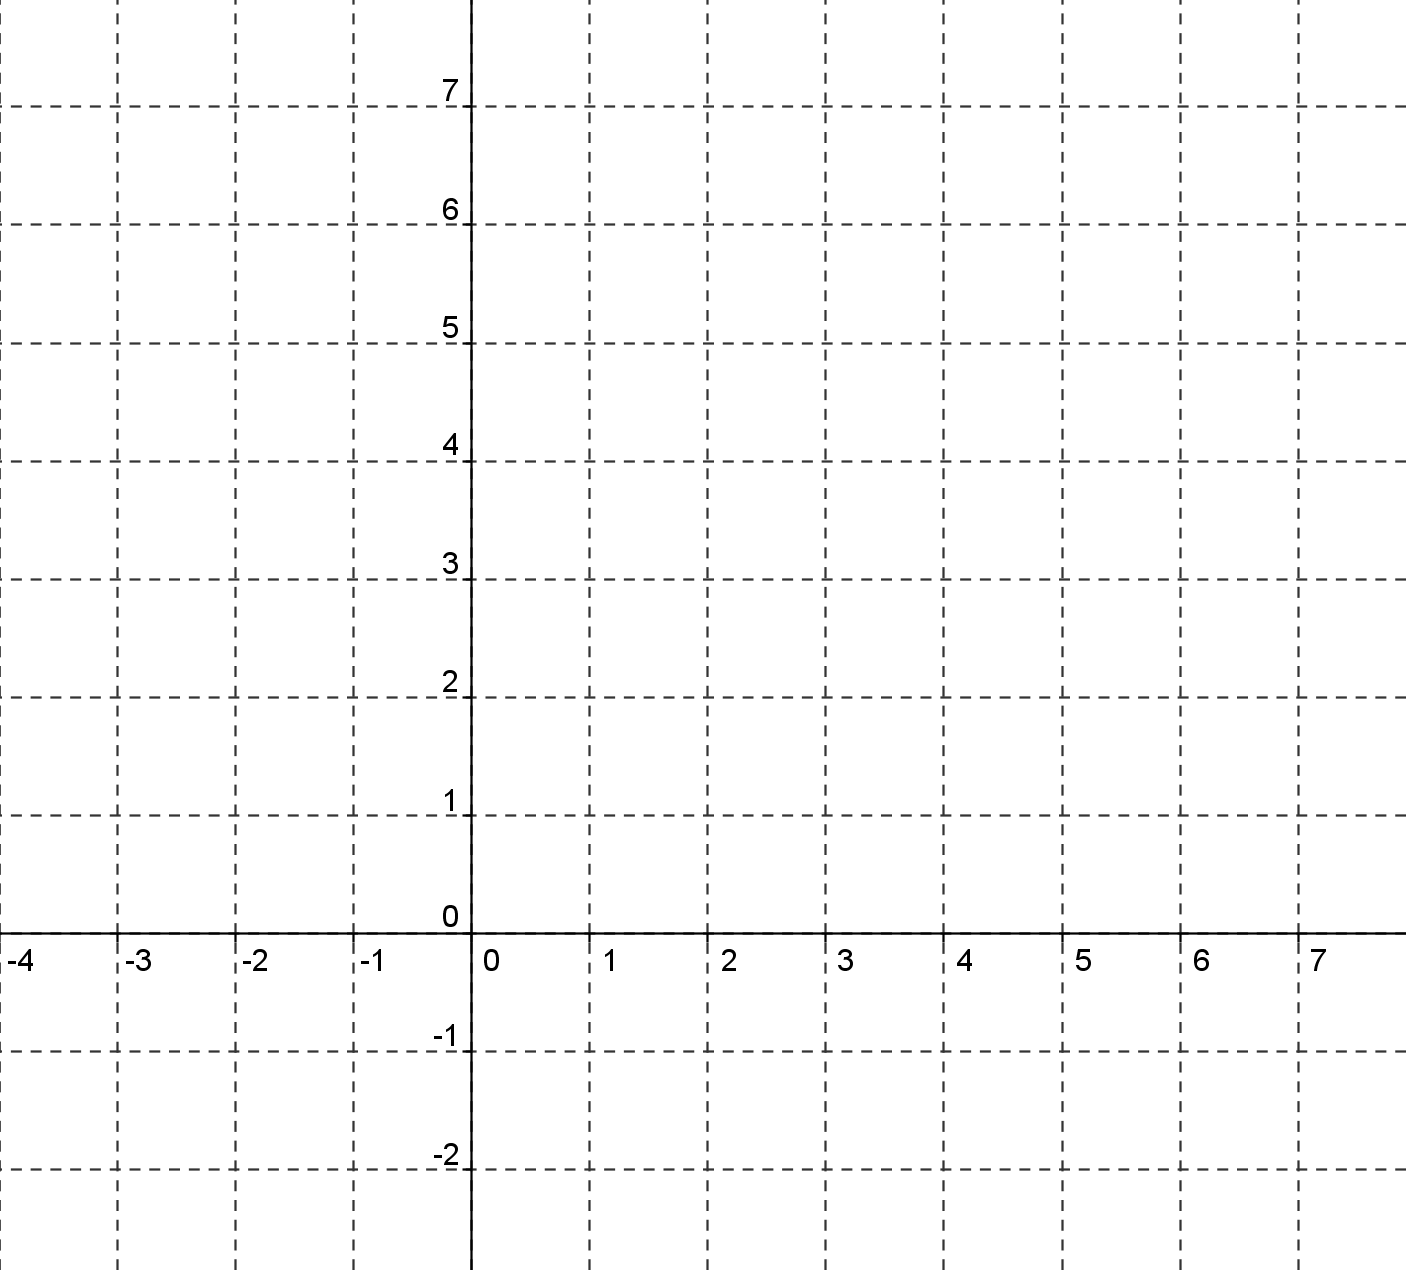
\includegraphics[width=12cm]{images/ex2.png}
\end{document}
